\documentclass{report}
\usepackage[spanish]{babel}
\usepackage{natbib}
\usepackage{url}
\usepackage[utf8]{inputenc}
\usepackage{amsmath}
\usepackage{graphicx}
\graphicspath{{images/}}
\usepackage{parskip}
\usepackage{fancyhdr}
\usepackage{vmargin}
\usepackage{subfig}
\usepackage[hidelinks]{hyperref}
\usepackage{enumerate}
\usepackage[usenames]{color}
\usepackage{soul}
\usepackage{float}
\usepackage[T1]{fontenc}
\usepackage{verbatim}
\usepackage{multicol}
\usepackage{listings}
\usepackage{multirow}
\usepackage{booktabs}
\usepackage{moreverb} 

\setmarginsrb{2.5 cm}{2.5 cm}{2.5 cm}{2.5 cm}{1 cm}{1.5 cm}{1 cm}{1.5 cm}

\title{\textsc{Reporte Proyecto Requerimientos de Proceso de Viáticos}}
\author{Luis Angel Hernández Lázaro\\  Daniel Méndez Cruz. }
\date{\today}

\makeatletter
\let\thetitle\@title
\let\theauthor\@author
\let\thedate\@date
\makeatother

\pagestyle{fancy}
\fancyhf{}
\rhead{\theauthor}
\lhead{\thetitle}
\cfoot{\thepage}
\setcounter{secnumdepth}{5}

\begin{document}

%%%%%%%%%%%%%%%%%%%%%%%%%%%%%%%%%%%%%%%%%%%%%%%%%%%%%%%%%%%%%%%%%%%%%%%%%%%%%%%%%%%%%%%%%

\begin{titlepage}
	\centering
    \vspace*{0.5 cm}
    
    
    \begin{figure}
		\centering
		\subfloat{
			\label{logoCimat}
		    
\includegraphics[scale = 0.15]{images/0cover/logoCimat.png}
		}
	\end{figure}
    \textsc{\LARGE Centro de Investigación en Matemáticas A.C.}\\[1.0 cm]
	\textsc{\Large Maestría en Ingeniería de Software}\\[0.5 cm]
	\textsc{\large Requerimientos de Ingeniería de Software\\Dr. Hugo Arnoldo Mitre}\\[0.5 cm]
	\rule{\linewidth}{0.2 mm} \\[0.4 cm]
	{ \huge \bfseries \thetitle}\\ \textsc{\large \\ Luis Angel Hernández Lázaro \\ Daniel Méndez Cruz}
	\rule{\linewidth}{0.2 mm} \\[1.5 cm]
	
	\begin{minipage}{0.5\textwidth}
		\begin{flushleft} \large
			\emph{Correo:}\\
			daniel.mendez@cimat.mx
		\end{flushleft}
	\end{minipage}~
	\begin{minipage}{0.4\textwidth}
		\begin{flushright} \large
			\emph{Correo:} \\
			luis.hernandez@cimat.mx
		\end{flushright}
	\end{minipage}\\[2 cm]
		
	{\large \thedate}\\[2 cm]
 
	\vfill
	
\end{titlepage}

%%%%%%%%%%%%%%%%%%%%%%%%%%%%%%%%%%%%%%%%%%%%%%%%%%%%%%%%%%%%%%%%%%%%%%%%%%%%%%%%%%%%%%%%%

\tableofcontents
\pagebreak

%%%%%%%%%%%%%%%%%%%%%%%%%%%%%%%%%%%%%%%%%%%%%%%%%%%%%%%%%%%%%%%%%%%%%%%%%%%%%%%%%%%%%%%%%
\chapter{Identificación del Problema}
    
    \section{Introducción}

En el problema que se abordó sobre el casos de uso, fue sobre las actividades que realizá \textbf{Jessica Garrido Sánchez}  quien se encarga de la administración y tramitar de las comisiones que los investigadores realizan en la temporada escolar. Ella es la encargada de gestionar todos los requisitos y documentos que se necesitan para que los investigadores realicen sus comisiones con los recursos necesarios, y de esa forma tener comprobantes de gastos que ellos le proveerán en el momento de su retorno.\\\\
Al principio ellos llenan un cuestionario que sirve como base para poder generar el oficio de comisión que será validadp por \textbf{Jessica} la cuál lo turna al Director de Cimat el Dr. \textbf{Cuauhtémoc Lemus}.\\\\
Previamente se generá una relación de gastos o una solicitud de fondos dependiendo de la opción que el investigador haya tomado previamente.\\\\
Una vez realizado este movimiento se procede al envío de la documentación a Guanajuato los cuales consisten en Oficio de comisión, relación de gastos e informe de comisión, estos documentos se envían tanto electrónico como físico.\\\\
Después de los trámites realizados sólo queda esperar que Cimat Guanajuato corrobore los documentos y los montos declarados en ellos para hacer efectivos los depósitos en las cuentas de los investigadores.\\\\
Cabe aclarar que para enviar los documentos a Guanajuato el Dr.\textbf{Cuauhtémoc Lemus} se encarga de firmar ya sea la solicitud de fondos o la relación de gastos para que pueda ser depósitado a los Investigadores a tiempo y conforme a la ley organica de la institución. 

\chapter{Análisis del Problema}

    \section{Introducción}
    En esta sección del trabajo se encuentran descritos los artefactos creados para visualizar el análisis de los requerimientos,entre los artefactos que se han creado se encuentran: \emph{Historias de Usuario}, \emph{Diagrama de Casos de Uso}, \emph{Diagrama de BPMN (Business Process Model and Notacion)} y el \emph{Diagrama de Clases}.\\ 
    Las \emph{Historias de Usuario} son empleadas para describir una funcionalidad que es de gran valor para el usuario del sistema. Son Utilizadas para permitir la comprensión por parte de todo el equipo de desarrollo involucrado, además ayudan  a tener una planificación eficaz.\\
    
    
    \section{Historias de Usuario}
    A continuación se presentan las Historias de Usuario Identificadas como requerimientos para el usuario.
    
    \fbox{\parbox[b]{\linewidth}{
        \begin{description}
            \item[<<Etiqueta>>]: HU1
            \begin{description}
                \item[``Yo como]: Asistente
                \item[quiero]: Obtener información especifica de los Investigadores
                \item[para]: 'poder generar el oficio de comisión '.
            \end{description}
            \item[<<Fecha>>]: 8-Dic-15
            \item[<<Responsable>>]: Jessica Garrido Sánchez
        \end{description}
    }}
    
    \fbox{\parbox[b]{\linewidth}{
        \begin{description}
            \item[<<Etiqueta>>]: HU2
            \begin{description}
                \item[``Yo como]: Asistente
                \item[quiero]: Generar oficio de comisión
                \item[para]: 'reembolsar gastos de los Investigadores'.
            \end{description}
            \item[<<Fecha>>]: 8-Dic-15
            \item[<<Responsable>>]: Jessica Garrido Sánchez
        \end{description}
    }}
    
    \fbox{\parbox[b]{\linewidth}{
        \begin{description}
            \item[<<Etiqueta>>]: HU3
            \begin{description}
                \item[``Yo como]: Investigador
                \item[quiero]: Llenar el cuestionario de datos
                \item[para]: 'Obtener el oficio de comisión'.
            \end{description}
            \item[<<Fecha>>]: 8-Dic-15
            \item[<<Responsable>>]: Investigador (es)
        \end{description}
    }}
    
    \fbox{\parbox[b]{\linewidth}{
        \begin{description}
            \item[<<Etiqueta>>]: HU4
            \begin{description}
                \item[``Yo como]: Asistente
                \item[quiero]: Validar oficio de comisión
                \item[para]: 'tener calidad en el tramite de comisión'.
            \end{description}
            \item[<<Fecha>>]: 8-Dic-15
            \item[<<Responsable>>]: Jessica Garrido Sánchez
        \end{description}
    }}

    \fbox{\parbox[b]{\linewidth}{
        \begin{description}
            \item[<<Etiqueta>>]: HU5
            \begin{description}
                \item[``Yo como]: Director
                \item[quiero]: comrpobar fondos 
                \item[para]:'Aprobar las solicitudes de comisión'.
            \end{description}
            \item[<<Fecha>>]: 8-Dic-15
            \item[<<Responsable>>]: Dr.Cuauhtémoc Lemus
        \end{description}
    }}
    
    
    \fbox{\parbox[b]{\linewidth}{
        \begin{description}
            \item[<<Etiqueta>>]: HU6
            \begin{description}
                \item[``Yo como]: Director
                \item[quiero]: Autorizar los oficios de comisión 
                \item[para]:  'que los Investigadores tengas la comisión'.
            \end{description}
            \item[<<Fecha>>]: 8-Dic-15
            \item[<<Responsable>>]: Dr. Cuauhtémoc Lemus
        \end{description}
    }}
    
    \fbox{\parbox[b]{\linewidth}{
        \begin{description}
            \item[<<Etiqueta>>]: HU7
            \begin{description}
                \item[``Yo como]: Investigador
                \item[quiero]: Entregar comprobantes 
                \item[para]: 'devolver dinero que se gastó en la comisión'.
            \end{description}
            \item[<<Fecha>>]: 8-Dic-15
            \item[<<Responsable>>]: Investigadores
        \end{description}
    }}    
    
    \fbox{\parbox[b]{\linewidth}{
        \begin{description}
            \item[<<Etiqueta>>]: HU8
            \begin{description}
                \item[``Yo como]: Asistente
                \item[quiero]: Generar relación de gastos / solicitud de fondos 
                \item[para]: 'Enviar a firma'.
            \end{description}
            \item[<<Fecha>>]: 8-Dic-15
            \item[<<Responsable>>]: Jessica Garrido Sánchez
        \end{description}
    }}

    \fbox{\parbox[b]{\linewidth}{
        \begin{description}
            \item[<<Etiqueta>>]: HU9
            \begin{description}
                \item[``Yo como]: Director
                \item[quiero]: Firmar solicitud de fondos / relación de gastos 
                \item[para]: 'enviar a Guanajuato'.
            \end{description}
            \item[<<Fecha>>]: 8-Dic-15
            \item[<<Responsable>>]: Dr.Cuauhtémoc Lemus
        \end{description}
    }}
    
    \fbox{\parbox[b]{\linewidth}{
        \begin{description}
            \item[<<Etiqueta>>]: HU10
            \begin{description}
                \item[``Yo como]: Investigador
                \item[quiero]: Firmar el informe de comisión
                \item[para]: 'Reintregrar los gastos'.
            \end{description}
            \item[<<Fecha>>]: 8-Dic-15
            \item[<<Responsable>>]: Investigador (es)
        \end{description}
    }}
    
       
    \section{Diagrama de Casos de Uso}
    
    \begin{figure}[H]
		\centering
			\label{logoCimat}
		    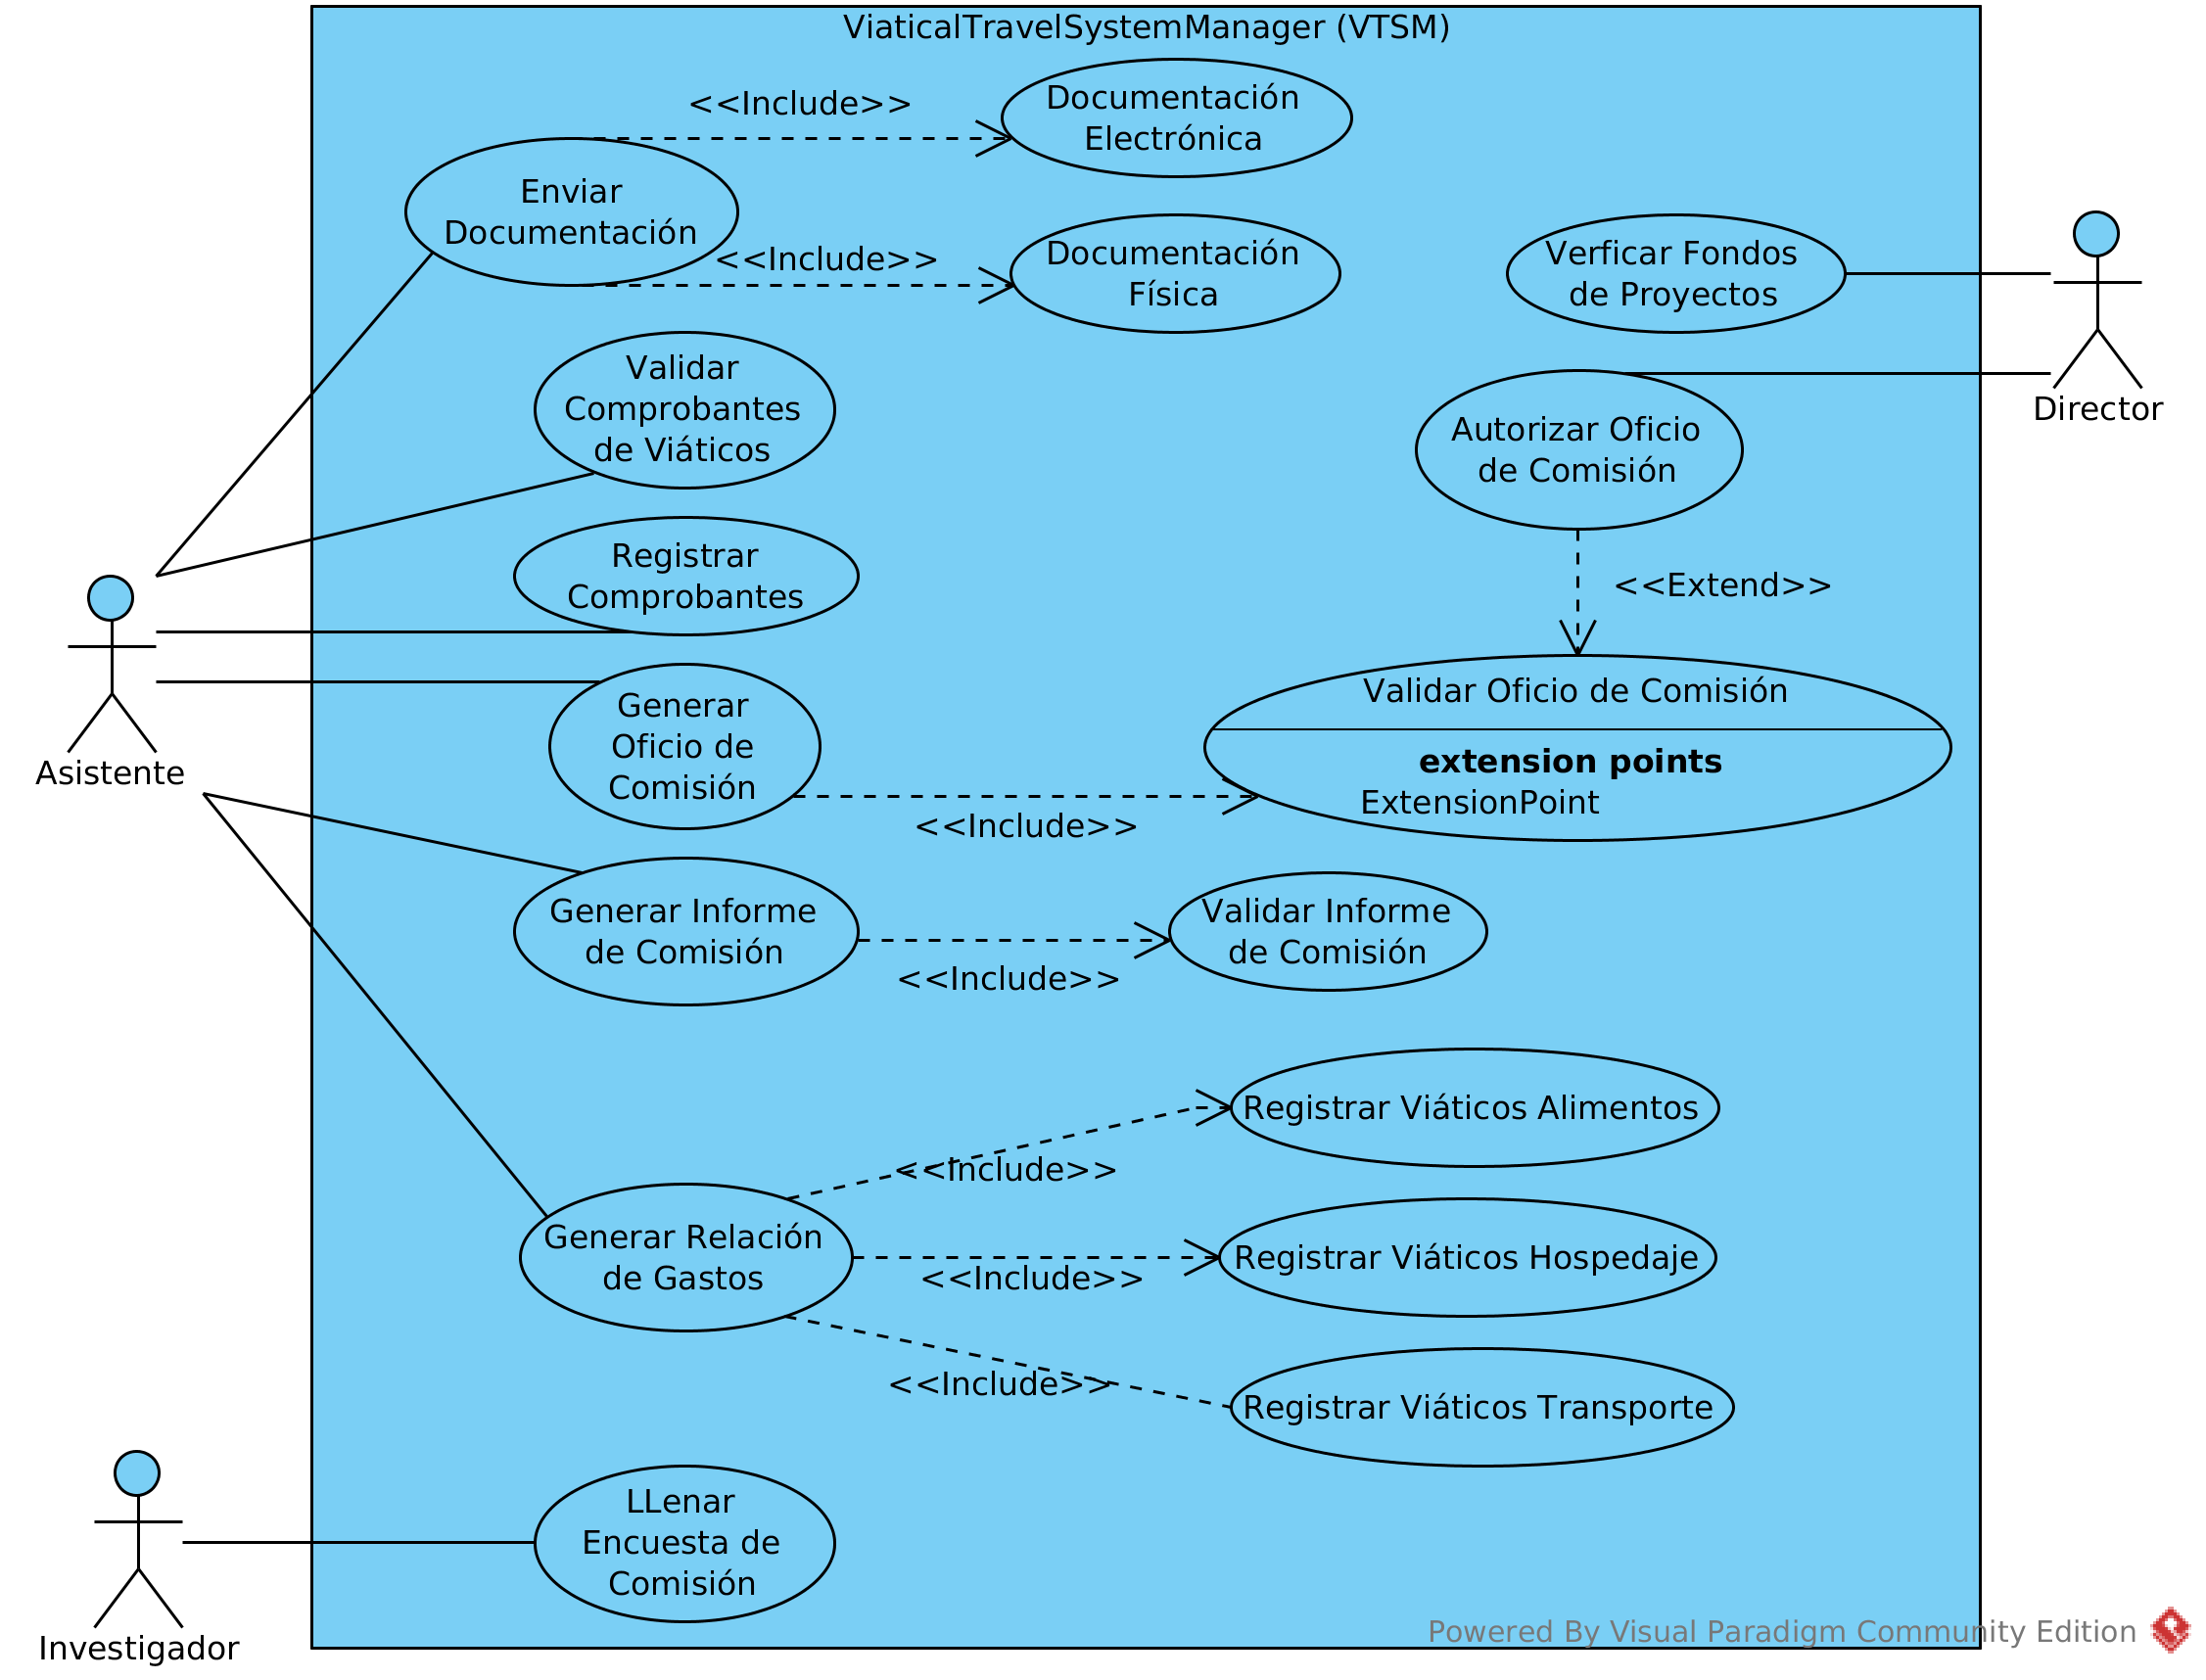
\includegraphics[scale = 0.80]{images/1models/useCase.png}
			\caption{Diagrama de Casos de Uso} 
	\end{figure}    
    
    \section{Diagrama BPMN (Business Process Model and Notacion)}
    
    	\begin{figure}[H]
    		\centering
    			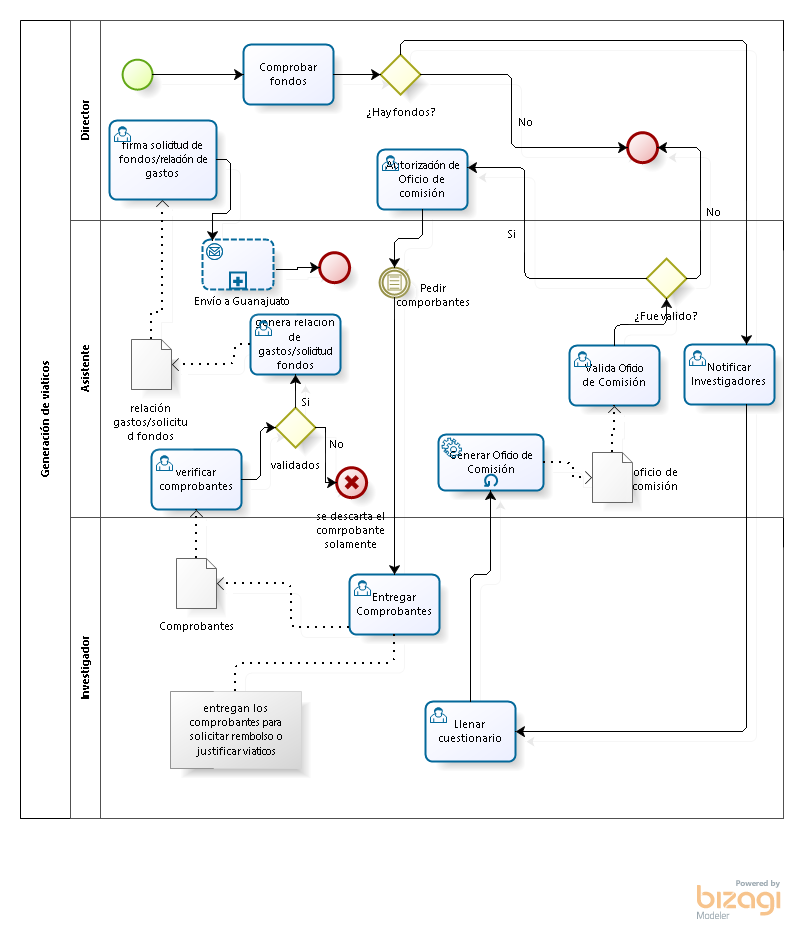
\includegraphics[scale=0.80]{images/1models/comision.png}  
    			\caption{Diagrama BPMN}  		
    	\end{figure}
    	
    	\begin{figure}[H]
    		\centering
    			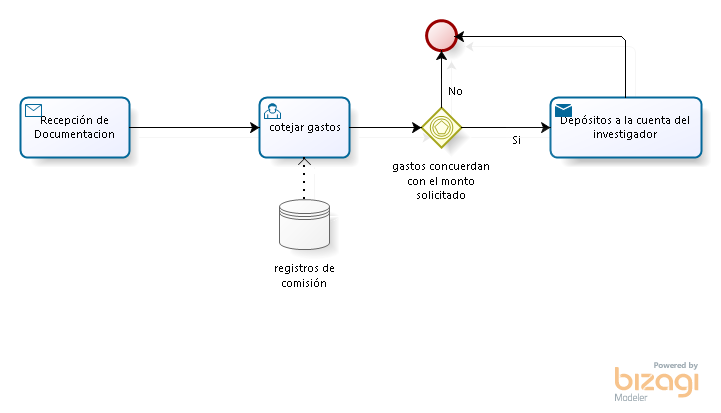
\includegraphics[scale=0.80]{images/1models/envioGto.png}
    			\caption{Diagrama BPMN Subproceso}
    	\end{figure}
    
    \section{Diagrama de clases}
    
    \section{Conclusiones}
       
\chapter{Lecciones Aprendidas de una Identificación de Requerimientos}
    
    \section{Lecciones Aprendidas}
    
    \section{Trabajos Futuros}
    
    \section{conclusiones}

\end{document}
